\documentclass{ssiBio}
\usepackage{siunitx}
\usepackage{verbatim}
\usepackage{graphicx}
\graphicspath{{images/}}

\title{Assay Development Proof of Concept I}
\author{Written by \textbf{Alan Tomusiak}}
\date{\textbf{Written:} May 21, 2019, \textbf{Performed:} May 23, 2019 - May 30, 2019, \textbf{Printed:} \today{}}
\begin{document}
\maketitle
\section{Procedure Purpose}
Perform a full validation of whether the technique employed by the assay development team is capable of testing backspace synthesis. Test every step in the assay to troubleshoot any problematic components. Determine whether a 5-bp or a 6-bp complementary strand will lead to more efficient nucleotide addition. Create positive and negative control results for future comparison.

\section{Overview}
In order to conduct DNA synthesis using water-soluble and non-toxic materials, a method using a pair of enzymes to extend and shorten a pre-existing template strand has been devised and termed the 'backspace' method. This technique involves three steps:
\begin{enumerate}
\item{Elongating an existing single-stranded DNA strand with an arbitrary length of one nucleotide of choice using Terminal Deoxynucleotidyl Transferase (TdT).}
\item{Adding a complementary strand that matches the 3' end of the original starting sequence, as well as one or two of the added nucleotides.}
\item{Introducing Exonuclease T, which will cleave the 3' region of the elongated starting strand, effectively cleaving excess nucleotides that are not to be added. \cite{zuo_deutscher_1999}}
\end{enumerate}
This experiment is intended to implement each of the steps of the 'backspace' technique, resulting in the addition of a single nucleotide to a pre-determined ssDNA strand. This is the first test of the AD assay, in which addition onto a pre-determined ~350bp strand is assayed using Sanger sequencing. The AD assay consists of the following:
\begin{enumerate}
\item{Creating a small 4-bp overhang on a template strand by using the BstXI restriction enzyme.}
\item{Performing backspace synthesis, as described above, on the template strand.}
\item{Poly-A tailing the template strand.}
\item{Creating a fully double-stranded sequence by filling in the single-stranded region using a Taq polymerase and an oligo d(T)18 primer.}
\item{Sanger sequencing the resulting strand.}
This experiment will also create positive and negative controls in order to better determine successful addition using the backspace synthesis method.
\end{enumerate}

\section{Safety Information}
\begin{safety}
  \begin{enumerate}
    \SYBRGOLD
  \end{enumerate}
\end{safety}

\section{Sample Explanations}
All samples will have R1-4 following them, indicating which replicate they belong to. Each sample and control will have four replicates.
\begin{enumerate}
  \item{\textbf{AD5}, Assay Development 5 - Sample testing the entirety of the backspace synthesis method using a complementary strand consisting of five basepairs.}
  \item{\textbf{AD6}, Assay Development 6 - Sample testing the entirety of the backspace synthesis method using a complementary strand consisting of six basepairs.}
  \item{\textbf{ADNC}, Assay Development Negative Control - Control designed to generate Sanger sequencing reads without backspace synthesis.}
  \item{\textbf{ADPC}, Assay Development Positive Control - Control designed to generate Sanger sequencing reads designed to imitate successful single basepair addition.}
\end{enumerate}

\section{Materials}
\begin{itemize}
  \item{BstXI-Digested, Verified AD Template}
  \item{Verified AD Positive Control}
  \item{100\uM{} Dev\_Seq\_Fwd2 Primer}
  \item{100\uM{} Dev\_Comp\_5\_Pure Primer}
  \item{100\uM{} Dev\_Comp\_6\_Pure Primer}
  \item{Agarose}
  \item{6X Purple Loading Dye}
  \item{1X Tris-Borate-EDTA (TBE) Buffer}
  \item{10,000X SYBR Green I}
  \item{Thermocycler}
  \item{30U/\uL{} Terminal Deoxynucleotidyl Transferase}
  \item{5X TdT Buffer}
  \item{Exonuclease T}
  \item{NEBuffer 4}
  \item{EDTA}
  \item{Qiagen PCR Purification Kit}
  \item{100mM dATP}
  \item{100mM dTTP}
  \item{10mM dNTPs}
  \item{10X Taq Reaction Buffer Pack}
  \item{Oligo d(T)18 Primer}
  \item{Goldbio 50bp DNA Ladder}
\end{itemize}

\section{Procedure}
\subsection{TdT Poly-T Tailing}
\begin{enumerate}
  \item{Dilute verified and purified BstXI-digested template DNA to a concentration of 25ng/\uL{}.}
  \item{Label twelve tubes as per the following:}
  \begin{enumerate}
    \item{AD5 R1 - AD5 R4}
    \item{AD6 R1 - AD6 R4}
    \item{ADNC R1 - ADNC R4}
  \end{enumerate}
  \item{Into the AD5 and AD6 tubes, pipette the following:}
  \begin{enumerate}
    \item{18.5\uL{} nuclease-free water.}
    \item{20\uL{} template DNA.}
    \item{10\uL{} 5X TdT Buffer.}
    \item{1\uL{} 100mM dTTP.}
    \item{.5\uL{} 30U/\uL{} Terminal Deoxynucleotidyl Transferase.}
  \end{enumerate}
  \item{Incubate at 37\C{} for an hour.}
  \item{Stop the reaction by heating at 70\C{} for ten minutes.}
  \stopPoint{}
  \item{Purify the reaction using a Qiagen PCR Purification kit. Dilute in 30 \uL{} of elution buffer for the final elution step.}
  \stopPoint{}
  \item{Run 2\uL{} of the reaction on a 2\% agarose gel. Run the gel according to the following table. Ensure that strands are uniformly tailed and that there is not a significant portion of template that is not tailed. If tailing is not complete, proceed to the next step and then repeat TdT tailing.}
    \begin{table}[ht]
    \centering
    \begin{tabular}{|l|l|}
    \hline
    \multicolumn{1}{|c|}{\textbf{Lane}} & \multicolumn{1}{c|}{\textbf{Sample}} \\ \hline
    1 & 50bp DNA Ladder \\ \hline
    2 & AD5 R1 \\ \hline
    3 & AD5 R2 \\ \hline
    4 & AD5 R3 \\ \hline
    5 & AD5 R4 \\ \hline
    6 & AD6 R1 \\ \hline
    7 & AD6 R2 \\ \hline
    8 & AD6 R3 \\ \hline
    9 & 10ng/uL Un-Digested Template \\ \hline
    10 & 10ng/uL Digested Template \\ \hline
    \end{tabular}
    \caption{\label{tab:gel-1-table}Gel 1 Loading Table.}
    \end{table}
  \item{To load the gel, mix the following on a piece of parafilm and then load 10\uL{} onto the gel lane:}
  \begin{itemize}
    \item{For the ladder lane, mix 5\uL{} of the ladder mix with 7\uL{} of 1X TBE buffer.}
    \item{For the remaining lanes, mix 3\uL{} of the sample with 7\uL{} of 1X TBE buffer and 2\uL{} of 6X Purple Loading Dye.}
  \end{itemize}
  \item{Run the gel at 100V until the lower loading dye marker is approximately halfway down the gel.}
  \stopPoint{}
  \item{Measure DNA concentration using a NanoDrop Spectrophotometer.}
  \item{Dilute DNA samples so that they have an even concentration according to the NanoDrop Spectrophotometer. To do this, dilute add water to all samples until they
  match the concentration of the sample that has the lowest concentration when measured by the NanoDrop.}
  \stopPoint{}
\end{enumerate}

\subsection{Complementary Strand Binding and Exonuclease T Cleavage}
\begin{enumerate}
\item{Into the AD5 tubes, add the following:}
\begin{enumerate}
  \item{5\uL{} NEBuffer 4.}
  \item{20\uL{} TdT-extended template.}
  \item{1.22\uL{} 100\uM{} Dev\_Comp\_5\_Pure.}
  \item{22.78\uL{} nuclease-free water.}
\end{enumerate}
\item{Into the AD6 tubes, add the following:}
\begin{enumerate}
  \item{5\uL{} NEBuffer 4.}
  \item{20\uL{} TdT-extended template.}
  \item{1.2\uL{} 100\uM{} Dev\_Comp\_6\_Pure.}
  \item{22.8\uL{} nuclease-free water.}
\end{enumerate}
\item{Place all eight tubes into a thermocycler.}
\item{Set the thermocycler to hold at 94\C{} for two minutes, and then ramp down to 5\C{} forever at a rate of 5\C{} per minute.}
\item{Add 1\uL{} of Exonuclease T to each tube, and allow incubation at 5\C{} for thirty minutes.}
\helpfulTip{For consistency between samples, it is important to perform the Exonuclease T addition step quickly. To make sure the temperature remains correct, keeping the thermocycler closed for as long as possible is essential.}
\item{Add 5\uL{} of 500mM EDTA to each tube. Mix. Heat inactivate by heating to 65\C{} for twenty minutes.}
\item{Run 4\uL{} of the reaction on a 2\% agarose gel. Run the gel according to the following table. Ensure that there is not a significant amount of tailed reaction left over. If there is a significant amount of tailed strand remaining, proceed to the next step and then repeat complementary strand binding and Exonuclease T cleavage.}
  \begin{table}[ht]
  \centering
  \begin{tabular}{|l|l|}
  \hline
  \multicolumn{1}{|c|}{\textbf{Lane}} & \multicolumn{1}{c|}{\textbf{Sample}} \\ \hline
  1 & 50bp DNA Ladder \\ \hline
  2 & AD5 R1 \\ \hline
  3 & AD5 R2 \\ \hline
  4 & AD5 R3 \\ \hline
  5 & AD5 R4 \\ \hline
  6 & AD6 R1 \\ \hline
  7 & AD6 R2 \\ \hline
  8 & AD6 R3 \\ \hline
  9 & AD6 R4 \\ \hline
  10 & 10ng/uL Digested Template \\ \hline
  \end{tabular}
  \caption{\label{tab:gel-2-table}Gel 2 Loading Table.}
  \end{table}
\stopPoint{}
\item{Purify the reaction using a Qiagen PCR Purification kit. Dilute in 40 \uL{} of elution buffer for the final elution step.}
\item{Measure DNA concentration using a NanoDrop Spectrophotometer.}
\stopPoint{}
\end{enumerate}

\subsection{Positive Control A-Overhang Addition}
\begin{enumerate}
\item{Label four tubes ADPC R1 - ADPC R4.}
\item{Dilute positive control template to a concentration of 25ng/\uL{}.}
\item{Dilute 100\uM{} dATP to a 10\uM{} concentration by adding 1\uL{} 100\uM{} dATP to 9\uL{} nuclease-free water.}
\item{Into the ADPC tubes, add the following:}
\begin{enumerate}
  \item{.25\uL{} Taq Polymerase.}
  \item{10\uL{} 25ng/\uL{} positive control template.}
  \item{5\uL{} 10X PCR buffer.}
  \item{1\uL{} 10\uM{} dATP.}
  \item{33.75\uL{} nuclease-free water.}
\end{enumerate}
\item{Incubate for 72\C{} for twenty minutes.}
\stopPoint{}
\item{Purify the reaction using a Qiagen PCR Purification kit. Dilute in 40 \uL{} of elution buffer for the final elution step.}
\item{Measure DNA concentration using a NanoDrop Spectrophotometer.}
\end{enumerate}
\stopPoint{}

\subsection{TdT Poly-A Tailing}

\subsection{Complementary Strand Fill-In}

\section{Results}
\begin{figure}[ht]
\centering
  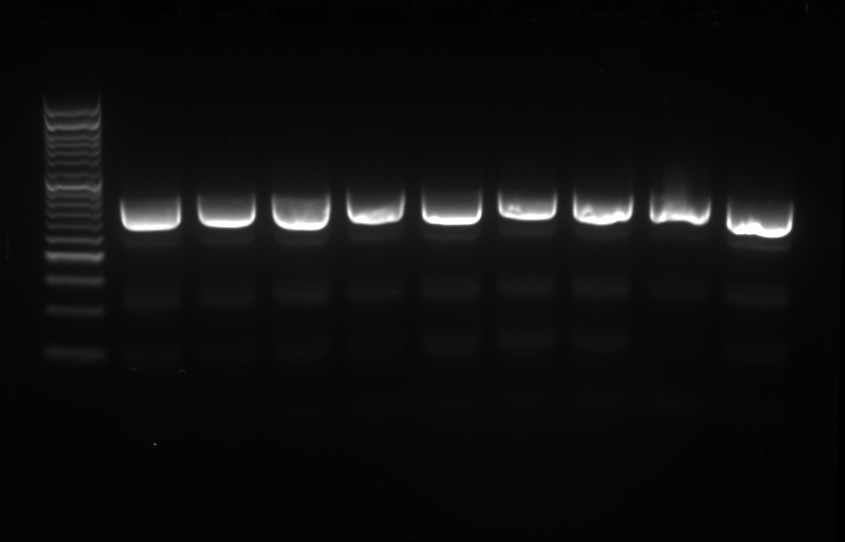
\includegraphics[width=.8\linewidth]{PCRAmplificationGel.png}
  \caption{Gel showing PCR-amplified template strands. Lane 1 is GoldBio 50bp Ladder, lanes 2-9 are randomly sampled PCR-amplified template strands.}
  \label{fig:figure1}
\end{figure}
\begin{figure}[ht]
\centering
  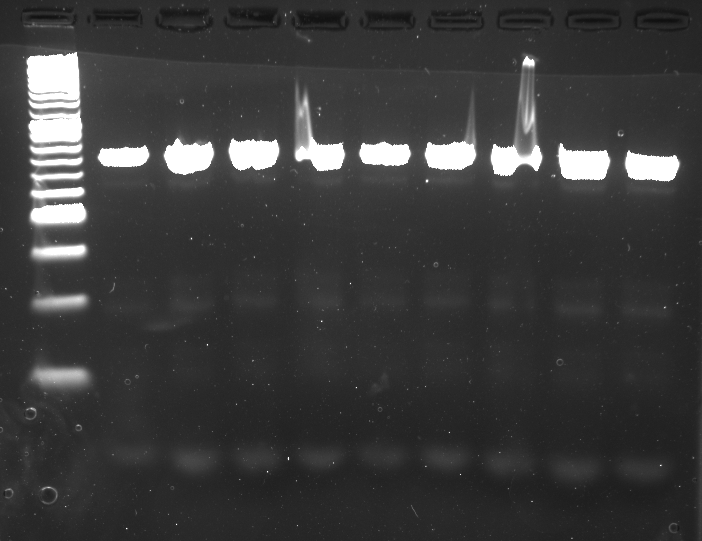
\includegraphics[width=.8\linewidth]{BstXIRestrictedGel.png}
  \caption{Gel showing PCR-amplified template strands. Lane 1 is GoldBio 50bp Ladder, lanes 2-9 are randomly sampled BstXI-digested template strands.}
  \label{fig:figure2}
\end{figure}
\begin{figure}[ht]
\centering
  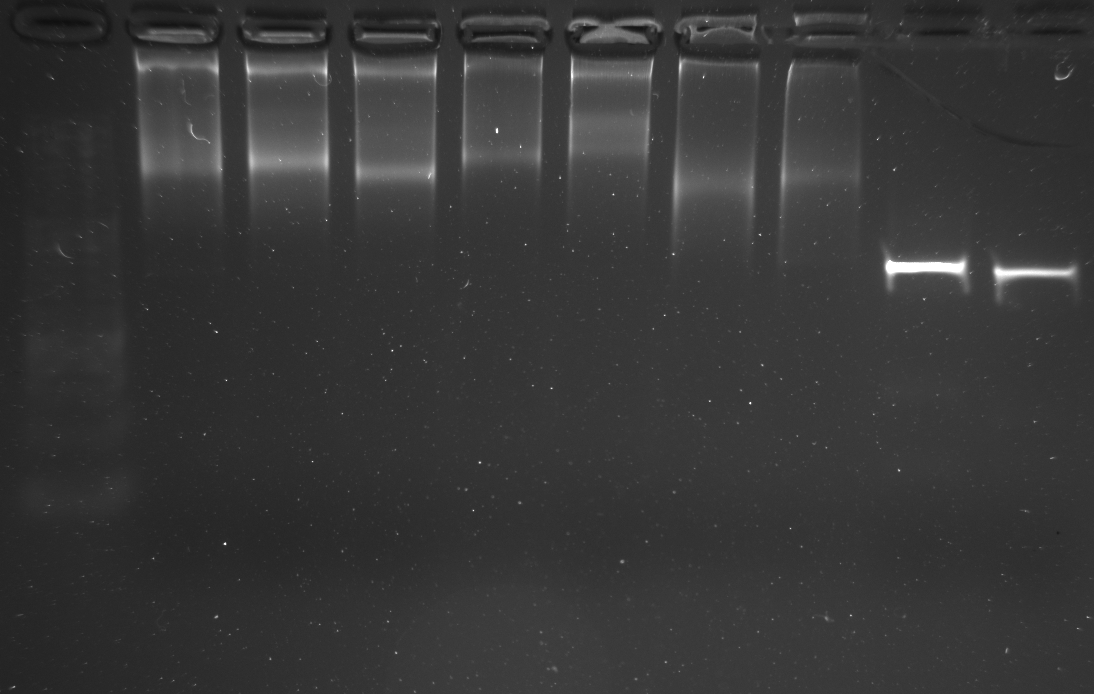
\includegraphics[width=.8\linewidth]{TdTTExtendedGel.png}
  \caption{Lanes correspond to Table 1 in `TdT Poly-T Tailing' section above.}
  \label{fig:figure3}
\end{figure}

\section{Analysis}

\section{Conclusions}

\bibliographystyle{ieeetr}
\bibliography{main}
\end{document}
